\chapter{Introducción}

\section{Importancia del ciclo día-noche en la evolución y desarrollo de la vida}

La duración del ciclo día-noche en la Tierra ha cambiado significativamente a lo largo de la historia geológica debido a la variación de la rotación del planeta. La velocidad de rotación original de los planetas  es consecuencia de la conservación del momento angular que poseía la nebulosa interestelar que, al colapsar, dio origen al Sistema Solar hace aproximadamente 4600 Ma \citep{Greaves2005}. Sin embargo, si la hipótesis del Impacto de Theia es correcta, es factible que la rotación primordial de la Tierra haya sido reconfigurada hace alrededor de 4500 Ma, cuando un cuerpo astronómico del tamaño de Marte, nombrado Theia, colisionó tangencialmente con nuestro planeta dando origen, además, a la Luna \citep{Stevenson1987}.\\

La masa lunar es lo suficientemente grande y cercana con respecto a la Tierra para ejercer atracción gravitatoria significativa sobre los océanos, generando así abultamientos de masas de agua (mareas) en ambos extremos del planeta alineados con el eje Tierra-Luna. Sin embargo, la rotación terrestre ocasiona el arrastre de las mareas hacia delante del mencionado eje, lo que implica que una fracción de la atracción gravitatoria Tierra-Luna está desfasada y da origen al torque lunar $\uptau_0$ que reduce la velocidad de rotación de la Tierra \citep{Conway1982}.\\ 

Como se muestra en la Figura~\ref{duraciondia}, la duración que tuvo el día terrestre posterior a la gran colisión de Theia debió de ser de tan sólo 7 horas aproximadamente gracias a la gran velocidad de rotación y el cambio en la inclinación del eje de rotación que el planeta llegó a experimentar luego del evento \citep{Stevenson&Bartlett2016}, \citep{Stevenson1987}; con el paso de los millones de años, tal velocidad fue disminuyendo como consecuencia del torque lunar \citep{Conway1982}.\\ 

El periodo estable de duración del día terrestre de 21 horas que se mantuvo durante gran parte del Precámbrico (Figura~\ref{duraciondia}) se explica con la llamada Hipótesis de Estabilización Resonante \citep{Zahnle&Walker1987}, la cual sostiene que, durante algún tiempo, el anteriormente mencionado torque lunar pudo haber sido cancelado por un torque de signo contrario originado por la resonancia entre las mareas atmosféricas semi-diurnas térmicamente accionadas y las oscilaciones libres de la atmósfera.\\

\begin{figure}
  \centering
    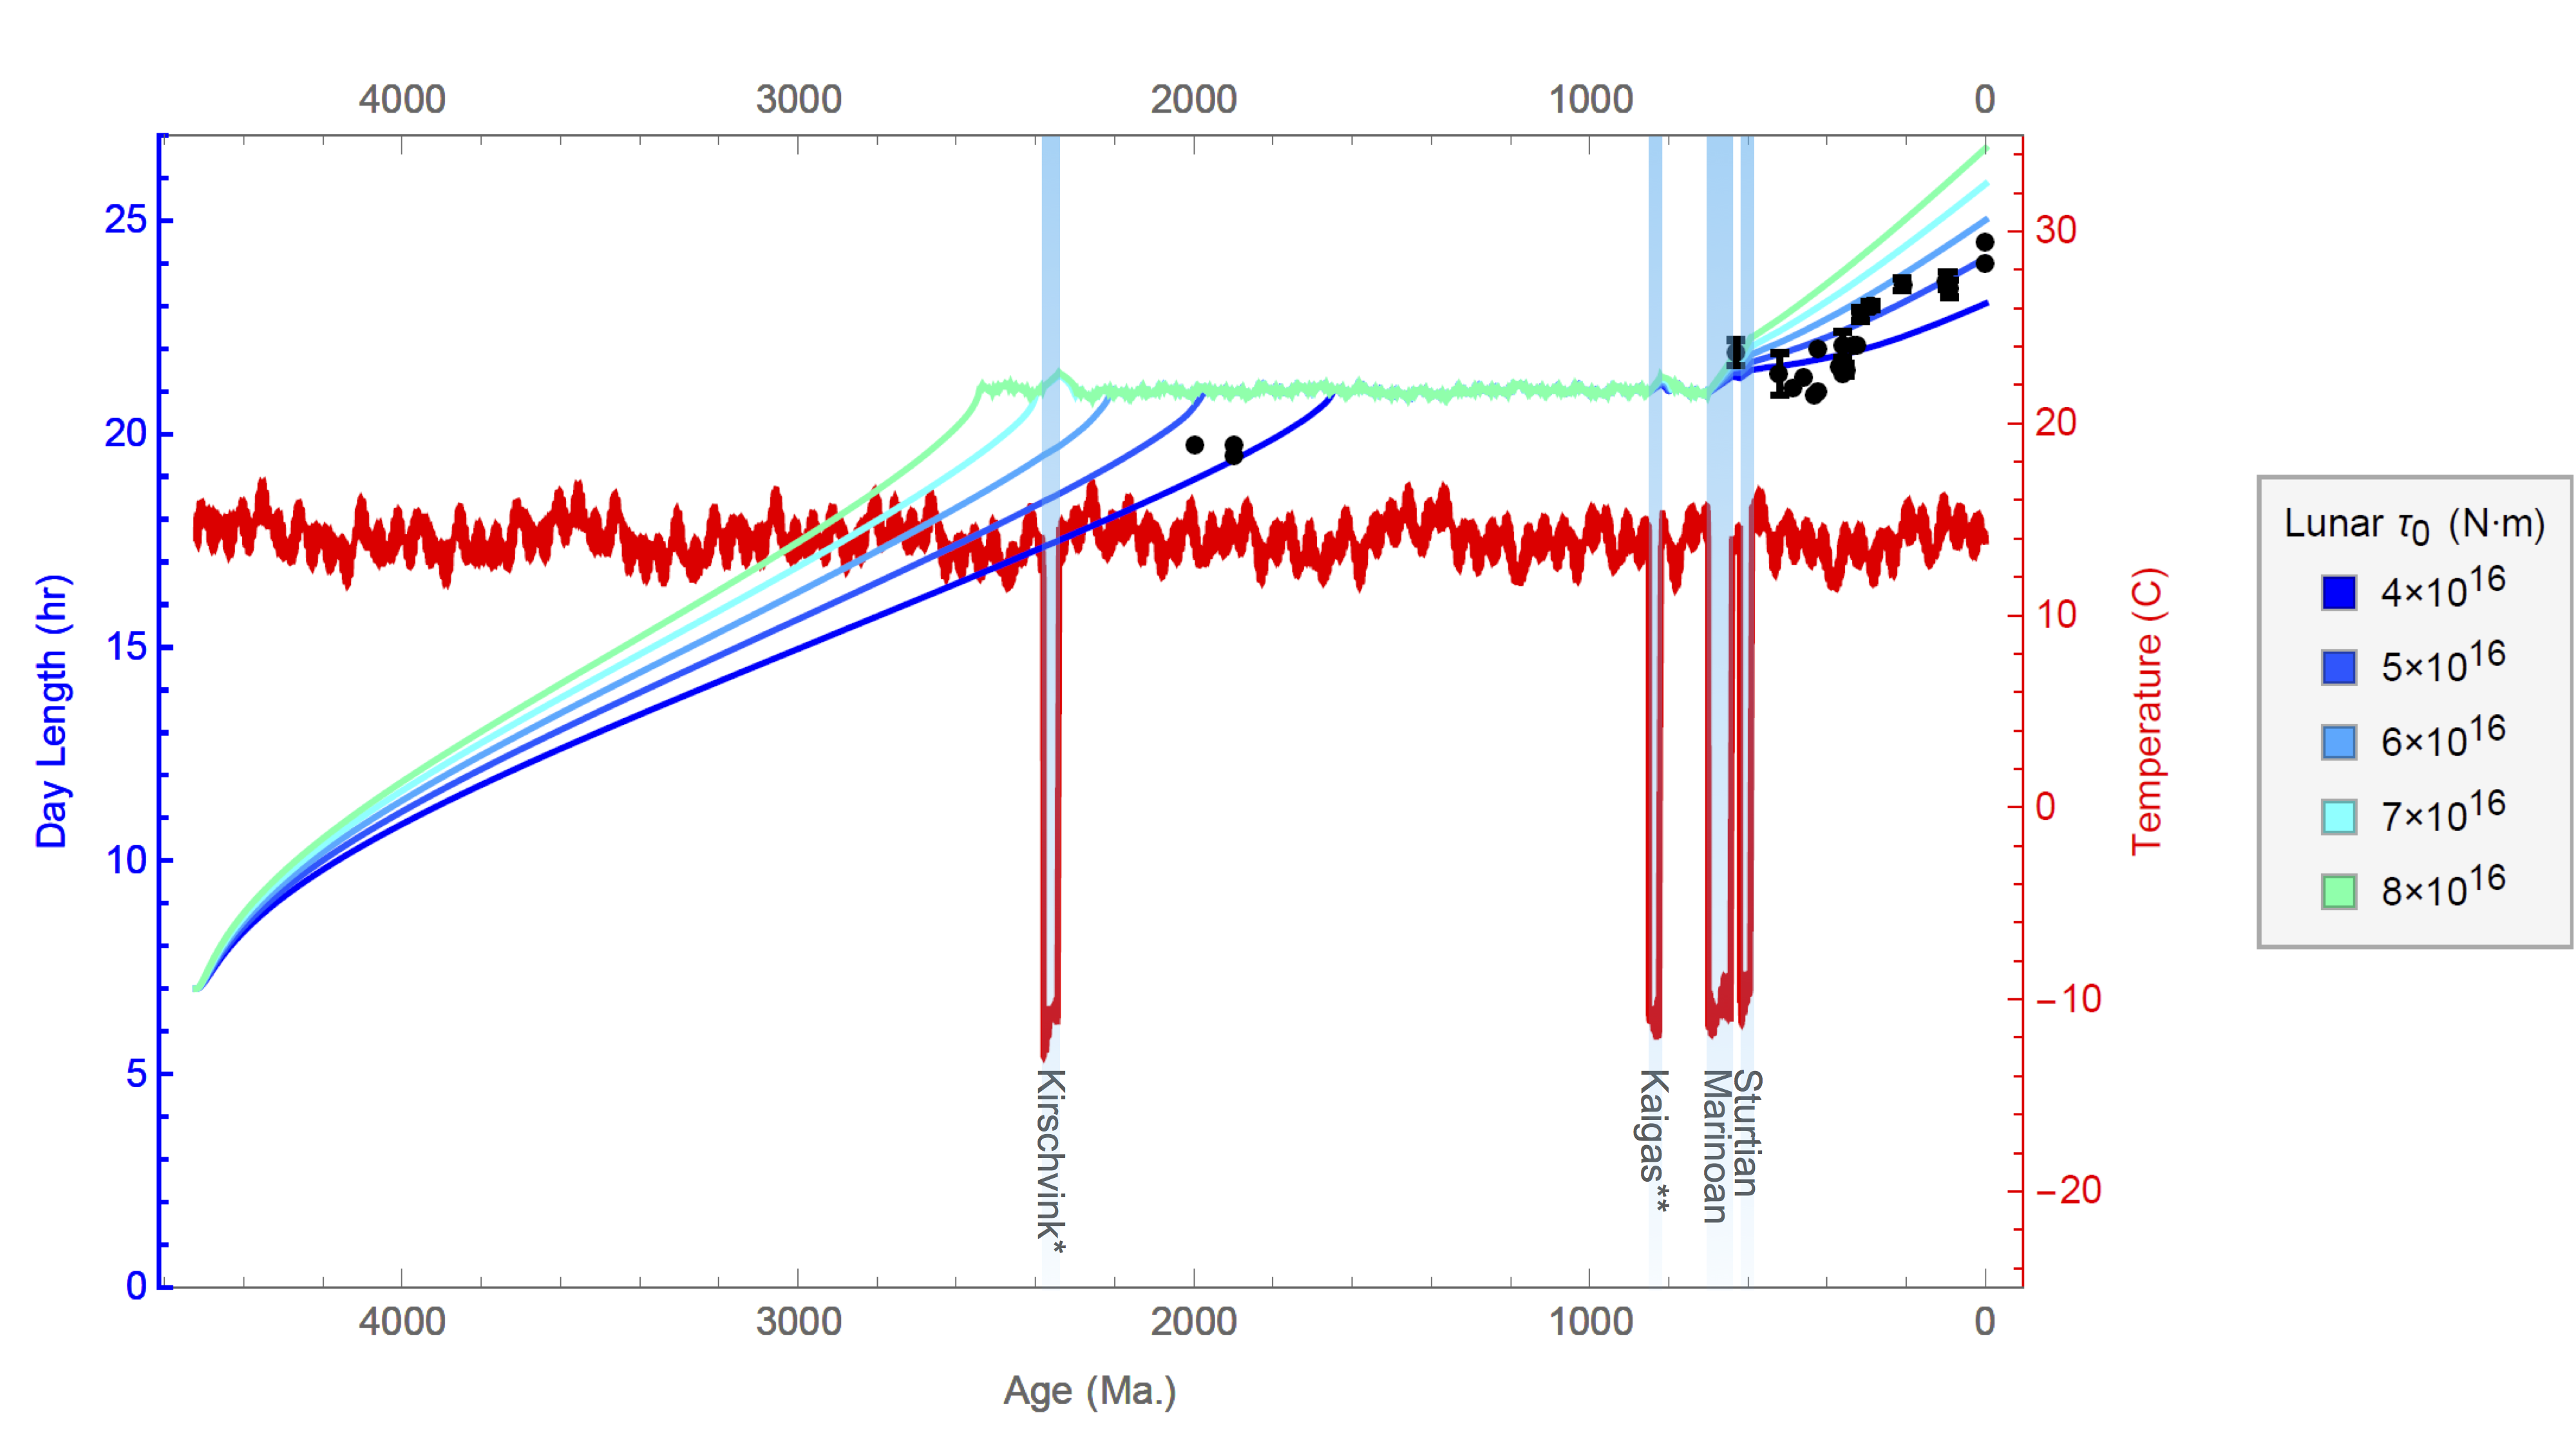
\includegraphics[width=1\textwidth]{duraciondeldiahistorico}
  \caption{Simulación de la historia geológica de la duración del día terrestre \citep{Stevenson&Bartlett2016}}
  \label{duraciondia}
\end{figure}

La velocidad de rotación actual de la Tierra debió comenzarse a perfilar hace aproximadamente 600 Ma cuando las grandes glaciaciones de ese entonces pudieron haber desestabilizado térmicamente el torque atmosférico, por lo que actualmente, el torque lunar sigue siendo lo suficientemente considerable como para continuar disminuyendo la velocidad del planeta \citep{Stevenson&Bartlett2016}. Para el final del Criogénico, el ciclo día-noche tomó, finalmente, su configuración actual al mismo tiempo que los niveles de oxígeno y ozono estratosférico fueron óptimos para el surgimiento y desarrollo de vida más compleja (multicelular) en un evento conocido como \textit{la Radiación del Cámbrico}, durante el que se originaron y diversificaron la mayoría de los filos animales incluyendo el de los cordados, al que pertenecemos los humanos .\\

$https://en.wikipedia.org/wiki/Cambrian_explosion$	
Poner la gráfica de Holker. Oscuridad, ventaja evolutiva. Más horas de noche, mayor nocturnidad con el paso del tiempo.\\

\section{Contaminación lumínica: qué es, tipos, orígenes, consecuencias, contexto histórico y ético}

BUSCAR PÁGINA DE SOCIOECOSISTEMAS:

Biofísico, ecosistema, definición de sistema, energía, materia, IIES, 

De ecosistema a socioecosistema diseñado
como territorio del capital agroindustria

Sistemas socio-ecológicos: elementos teóricos y conceptuales para la discusión en torno a vulnerabilidad hídrica

Uso y abuso de la energía

\section{Brillo del cielo nocturno}

\subsection{Componentes del brillo del cielo nocturno}


De acuerdo con Leinert at.al (1998), el brillo total $(I_{tot})$ del cielo nocturno puede calcularse a partir de la siguiente ecuación:

\begin{equation}\label{eq:ej}
I_{tot}=(I_A + I_{ZL} + I_{ISL} + I_{DGL} + I_{EBL})\ exp \ (-\tau) + I_{SCA}
\end{equation}

Donde $\tau$ es el coeficiente de extinción que depende de la longitud de onda, el ángulo cenital, la altura sobre el nivel del mar y la composición atmosférica del lugar de la observación.


\subsection{Variación natural del brillo del cielo nocturno por influencia de objetos astronómicos}

\subsection{Variación natural del brillo del cielo nocturno por influencia de las condiciones atmosféricas}

\subsubsection{Propiedades ópticas de las nubes}

\subsubsection{Propiedades ópticas del aerosol atmosférico}


\section{Estudio de caso: Ciudad de México}

\subsection{Descripción del área de estudio}

Incluir REPSA

\subsection{Climatología de nubes y aerosol atmosférico en la Ciudad de México}